\subsection{Distancia euclidiana}
La distancia euclidiana es simplemente la distancia entre dos puntos cuando se calcula haciendo uso del teorema de Pitágoras. Viene dado por la raíz cuadrada de $(x_1 - x_2)^2 + (y_1 - y_2)^2$.

% TODO: \usepackage{graphicx} required
\begin{figure}[h!]
	\centering
	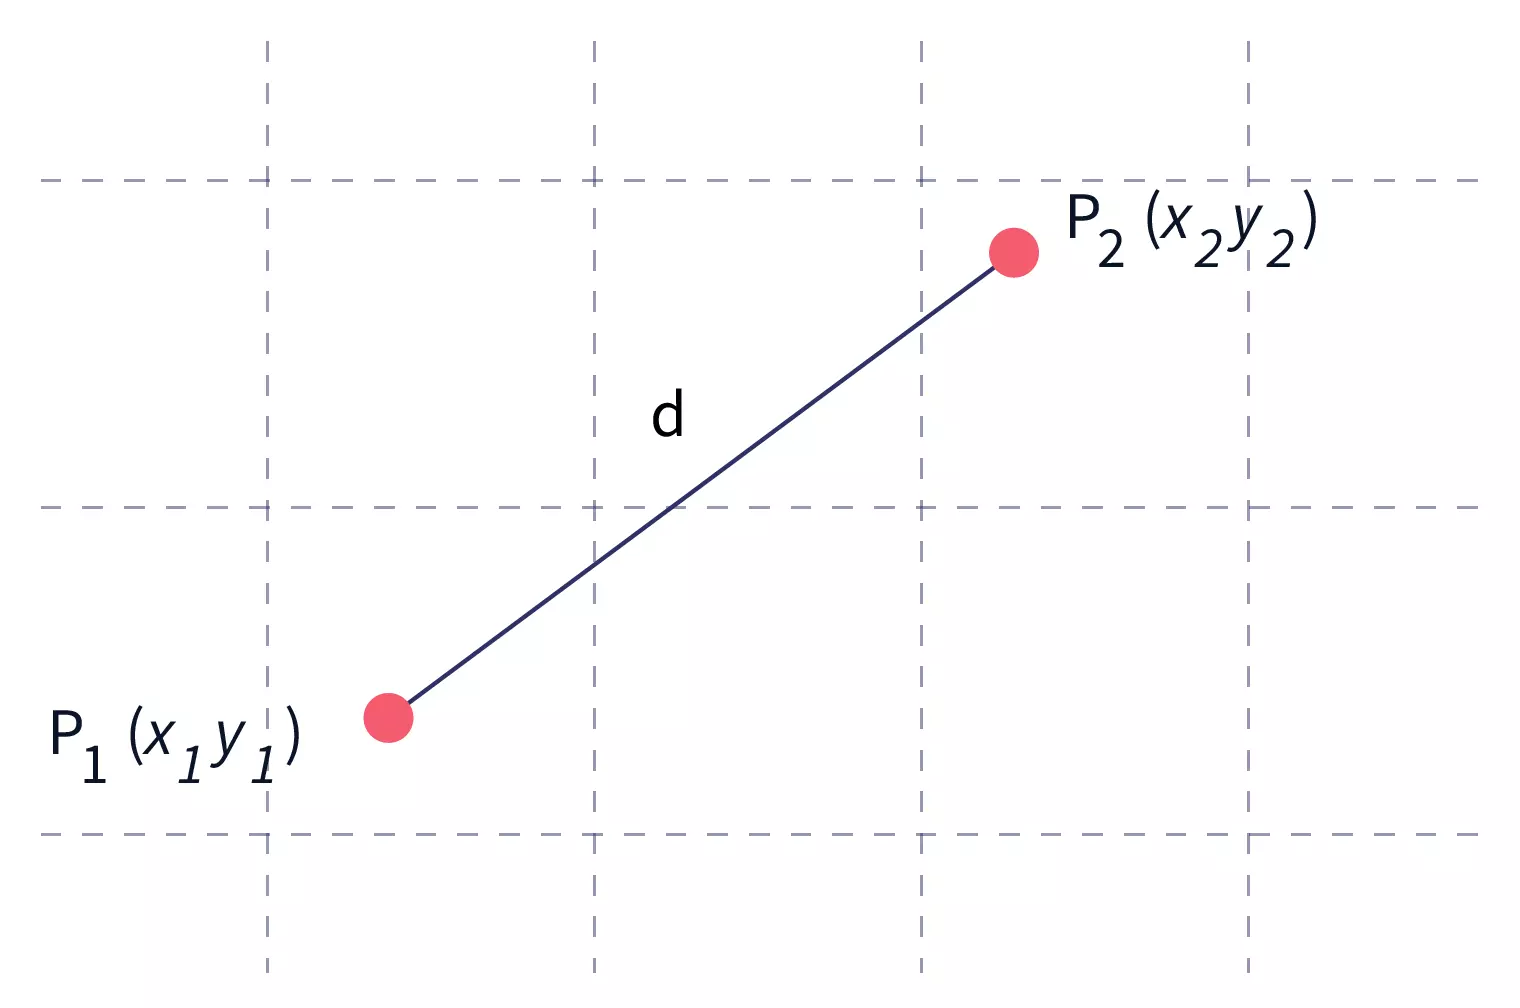
\includegraphics[width=0.35\linewidth]{img/distancia_euclidiana}
	\label{fig:distanciaeuclidiana}
\end{figure}


\subsection{Distancia Manhattan}
La distancia de Manhattan es la distancia recorrida cuando te mueves solo verticalmente o solo horizontalmente. Está dado por $ |x_1-x_2| + |y_1-y_2|$.

% TODO: \usepackage{graphicx} required
\begin{figure}[h!]
	\centering
	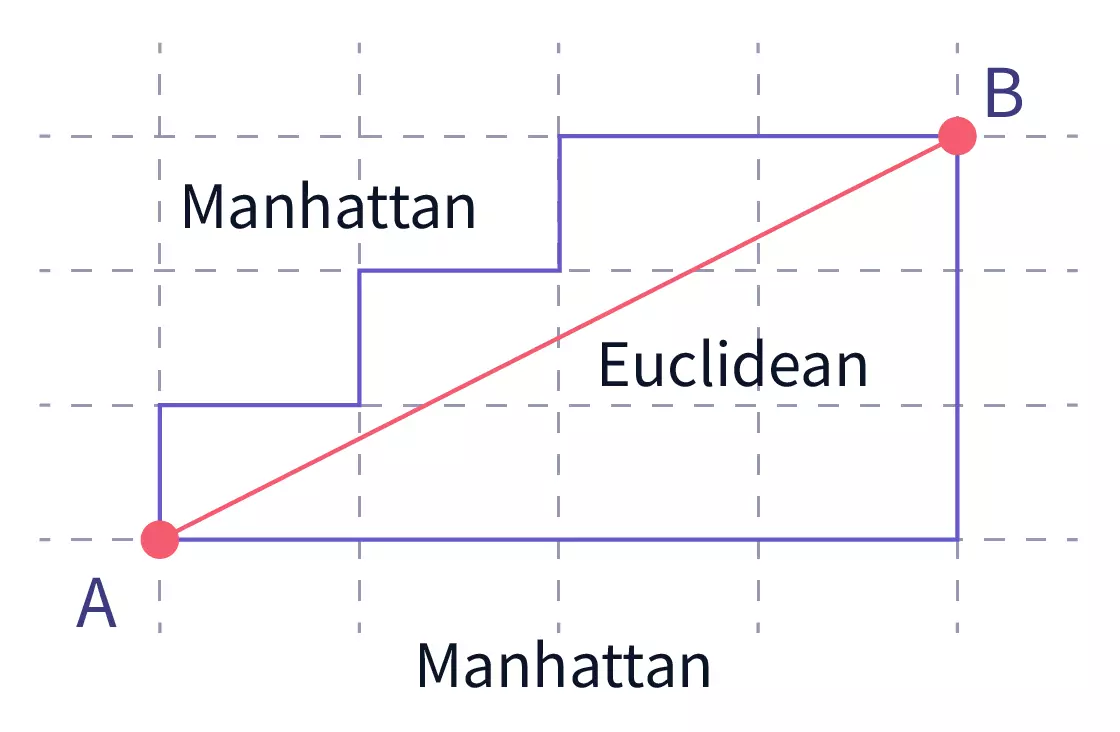
\includegraphics[width=0.35\linewidth]{img/distancia_manhattan}
	\label{fig:distanciamanhattan}
\end{figure}

\subsection{Árbol de expansión mínima}

Dado un grafo conexo y no dirigido, un árbol recubridor, árbol de cobertura o árbol de expansión de ese grafo es un subgrafo que tiene que ser un árbol y contener todos los vértices del grafo
inicial. Cada arista tiene asignado un peso proporcional entre ellos, que es un número representativo de algún objeto, distancia, etc.; y se usa para asignar un peso total al árbol recubridor mínimo
computando la suma de todos los pesos de las aristas del árbol en cuestión. Un árbol recubridor
mínimo o un árbol de expansión mínimo es un árbol recubridor que pesa menos o igual que todos
los otros árboles recubridores. Todo grafo tiene un bosque recubridor mínimo.
